\documentclass{scrartcl}

\usepackage{graphicx}
\usepackage[utf8]{inputenc}
\usepackage[T1]{fontenc}
\usepackage{lmodern}
\usepackage{babel}
\usepackage{amsmath}
\usepackage{amsthm}
\usepackage{mathtools}
\usepackage{amssymb}
\usepackage{listings}
\usepackage{xparse}
\usepackage{geometry}
\usepackage{enumerate}
\usepackage{tikz}
\usepackage[style=english]{csquotes}
\usepackage[language=english, backend=biber, style=alphabetic, sorting=nyt]{biblatex}

\usetikzlibrary{babel, positioning, shapes.geometric, arrows, arrows.meta}
\addbibresource{bibliography.bib}

\title{SIKE - A key exchange scheme based on Supersingular Elliptic Curves}
\author{Simon Pohmann}

\newcommand{\N}{\mathbb{N}}
\newcommand{\Z}{\mathbb{Z}}
\newcommand{\F}{\mathbb{F}}
\newcommand{\proj}{\mathrm{proj}}
\newcommand{\Quot}{\mathrm{Quot}}
\renewcommand{\O}{O}

\newtheorem{prop}{Proposition}[section]
\newtheorem{theorem}[prop]{Theorem}
\newtheorem{lemma}[prop]{Lemma}
\newtheorem{corollary}[prop]{Corollary}
\newtheorem{problem}[prop]{Problem}
\newtheorem{alg}[prop]{Algorithm}
\newtheorem{definition}[prop]{Definition}
\newtheorem{example}[prop]{Example}
\newtheorem{remark}[prop]{Remark}

\begin{document}

\maketitle

\tableofcontents

\section{Elliptic Curves as Varieties}

\subsection{Definition}

For this work, we define elliptic curves as certain varieties in the projective plane over $\bar{K}$ as follows.

\begin{definition}
    A (possibly nonsmooth) elliptic curve $E$ defined over a field $K$ is the (projective) zero set
    \begin{equation*}
        E = \mathcal{Z}_{\bar{K}}(Y^2Z + a_1 XYZ + a_3 YZ^2 - X^3 - a_2 X^2 Z - a_4 X Z^2 - a_6 Z^3) \subseteq \mathbb{P}_{\bar{K}}^2
    \end{equation*}
    of some irreducible polynomial $Y^2Z + a_1 XYZ + a_3 YZ^2 - X^3 - a_2 X^2 Z - a_4 X Z^2 - a_6 Z^3 \in K[X, Y, Z]$.
    The point $\O := (0 : 1 : 0) \in E$ is called the point at infinity of the elliptic curve.
\end{definition}

It is convention to define an Elliptic Curve by the dehomogenization
\footnote{For a homogeneous polynomial $f \in K[x, y, z]$ the dehomogenization is $f(x, y, 1)$, denoted by $f^{\mathrm{deh}}$.}  
of its defining polynomials, i.e. say that the curve $E$ is defined by the equation
\begin{equation*}
    E: \ Y^2 + a_1 XY + a_3 Y = X^3 + a_2 X^2 + a_4 X + a_6
\end{equation*}
which is also called Weierstraß equation of $E$.
By homogenizing the polynomial equation, one can retrieve the original homogeneous polynomial, so this representation defines the Elliptic Curve uniquely.

Readers that are not used to working with projective geometry may also think of an Elliptic Curve as the (affine) set of solutions of this equation, together with a dedicated point $\O$ ``at infinity''.
In this spirit, we will also identify affine points $(x, y)$ with $(x : y : 1)$.

Usually, one only considers elliptic curves that are smooth. 
This is a property that can be defined for all varieties, but here we will only give a definition applicable only to elliptic curves.
This relies on the so-called discriminant of an elliptic curve.

\begin{definition}
    \label{def:discriminant}
    A (possibly nonsmooth) elliptic curve $E$ defined by $Y^2 + a_1 XY + a_3 Y = X^3 + a_2 X^2 + a_4 X + a_6$ is called smooth, if the discriminant
    \begin{align*}
        \Delta(E) = & - b_2^2 b_8 - 8 b_4^3 - 27 b_6^2 + 9 b_2 b_4 b_6 \\
        \text{where} \quad & b_2 = a_1^2 + 4 a_2 \\
        & b_4 = a_1 a_3 + 2 a_4 \\
        & b_6 = a_3^2 + 4 a_6 \\
        & b_8 = a_1^2 a_6 + 4 a_2 a_6 - a_1 a_3 a_4 + a_2 a_3^2 - a_4
    \end{align*}
    is nonzero. In this work, the term ``elliptic curve'' will be used for smooth elliptic curves.
\end{definition}

One can now check by a lengthy computation that having a nonzero discriminant is equivalent to having a well-defined tangent line at every point.
For the sake of brevity, we will not perform the computation in this work.

\subsection{Isogenies}

In this section, we will introduce the notion of an isogeny, which are the structure-preserving maps between Elliptic Curves.
A crucial part of this definition are morphisms, which are the structure-preserving maps in the category of algebraic varieties.
Their theory is quite wide, and anything further than giving the definitions and some basic facts is beyond the scope of this work.
The interested reader is advised to refer to a book on Algebraic Geometry.
However, we try to give sufficient intuition that one can follow the rest of this work without a background in Algebraic Geometry.

\begin{definition}
    \label{def:rational_map}
    Given irreducible varieties $V = \mathcal{Z}_{\bar{K}}(I), W \subseteq \mathbb{P}_{\bar{K}}^2$, a partial map $\phi: V \to W$ is called rational if it is given locally by rational functions.
    Namely, $\phi$ is rational if there are homogeneous $f_1, f_2, f_3 \in \bar{K}[X, Y, Z]$ of same degree and not all zero such that for each point $(a_1 : a_2 : a_3) \in V$ at which $\phi$ is defined, there are ``equivalent'' homogeneous polynomials $(g_1, g_2, g_3) \in \bar{K}[X, Y, Z], \ (g_1, g_2, g_3) \sim (f_1, f_2, f_3)$ of same degree such that
    \begin{align*}
        (g_1(a), g_2(a), g_3(a)) &\neq (0, 0, 0) \quad \text{and}\\
        (g_1(a) : g_2(a) : g_3(a)) &= \phi((a_1 : a_2 : a_3))
    \end{align*}
    where $a = (a_1, a_2, a_3)$.

    Here we define equivalence as $(f_1, f_2, f_3) \sim (g_1, g_2, g_3)$ if $f_i g_j = f_j g_i \mod I$ for all $i, j$.
    We use the notation $\phi = [f_1^{\mathrm{deh}} / f_3^{\mathrm{deh}}, f_2^{\mathrm{deh}} / f_3^{\mathrm{deh}}, 1]$
    \footnote{Note that $f$ corresponds to $f^{\mathrm{deh}}$ uniquely except for scaling by $z$, but scaling by $z$ does not change the defined rational map. This ``affine'' notation corresponds to the use of dehomogenized polynomials for defining Elliptic Curves.}.
    The rational map is said to be defined over $K$, if $f_1, f_2, f_3 \in K[X, Y, Z]$.
\end{definition}

This definition is quite technical, as rational maps are defined locally.
The idea is that one considers different functions given by fractions of polynomials, each defined only on a subset of $E$ (i.e. excluding the cases where one would get ``$\frac 0 0$'' or ``$(0 : 0 : 0)$'').
We now get a rational map by ``gluing'' them together, i.e. define the value of the map as the value of an applicable function.
For the rational map to be well-defined, we thus require that on points where multiple functions are applicable, they yield the same value.

As these sets of definition, one allows only sets that are open in the Zariski topology.
As a result, their intersections are again open in the Zariski-topology, and thus already uniquely determine the polynomial.
It follows that all the polynomials that are glued together must be ``equivalent'' according to the above definition.

Note that we still defined rational maps as partial maps, i.e. although we use a local definition, it is possible that no value is defined for a certain point.
Rational maps that are not partial are then the ``nice'' maps of Algebraic Geometry.

\begin{definition}
    A rational map between varieties that is defined everywhere is called morphism. 
    If it is bijective and its inverse is a morphism, it is called a variety isomorphism.
\end{definition}

As we will see in the next part, Elliptic Curves contain more structure than just the geometric one.
Thus we will work with the stronger notion than that of a morphism.

\begin{definition}
    \label{def:isogeny}
    A morphism $\phi$ between Elliptic Curves $E_1, E_2$ is called isogeny, if $\phi(\O) = \O$.
    A bijective isogeny whose inverse is also an isogeny is called isomorphism.
\end{definition}

Similar to the convention of defining Elliptic Curves by dehomogenized polynomials, we will use a notation that does not rely on homogeneous coordinates.
For this, we require the coordinate ring of an Elliptic Curve, which is the ring of ``polynomial functions'' defined on the curve.

\begin{definition}
    Let $E$ be an Elliptic Curve defined by the polynomial $F(X, Y) = Y^2 + a_1 XY + a_3 Y - X^3 - a_2 X^2 - a_4 X - a_6$.
    Then the ring $K[E] := K[X, Y] / (F(X, Y))$ is called the (affine) coordinate ring of $E$.
    Its field of fractions is called the function field of $E$ and denoted by $K(E)$.
\end{definition}

\begin{prop}
    Let $E_1, E_2$ be Elliptic Curves and $\phi: E_1 \to E_2$ be a map with $\phi(\O) = \O$.
    Then the following are equivalent:
    \begin{itemize}
        \item $\phi$ is an isogeny
        \item There are elements $u, v \in \bar{K}(E)$ such that for all $a = (x, y) \in E$ there are polynomials $g_1, g_2, g_3 \in \bar{K}[X, Y]$ with
        \begin{equation*}
            \frac {\overline{g_1}} {\overline{g_3}} = u, \ \frac {\overline{g_2}} {\overline{g_3}} = v \quad \text{in $\bar{K}(E)$}
        \end{equation*}
        and
        \begin{equation*}
            g_3(a) \neq 0, \ \phi(a) = \Bigl( \frac {g_1(a)} {g_3(a)}, \frac {g_2(a)} {g_3(a)} \Bigr) \quad \text{or} \quad (g_1(a), g_2(a)) \neq (0, 0), \ \phi(a) = \O
        \end{equation*}
    \end{itemize}
    In this case $\phi = [u, v, 1]$.
\end{prop}
\begin{proof}
    For $\Leftarrow$ we have to show that $\phi$ is an isogeny, i.e. show the condition from \ref{def:rational_map}.
    Let $f_1, f_2, f_3 \in K[X, Y, Z]$ homogeneous of same degree such that $f_1^{\mathrm{deh}} / f_3^{\mathrm{deh}}$ is a representative of $u$ and $f_2^{\mathrm{deh}} / f_3^{\mathrm{deh}}$ is a representative of $v$.
    For a point $(x : y : z) \neq \O$ we have wlog that $z = 1$, so $(x : y : z) = (x, y)$.
    
    Let now be $g_1, g_2, g_3 \in K[X, Y]$ the polynomials given by the assumption and $d = \max \{ \deg g_1, \deg g_2, \deg g_3 \}$.
    Then the polynomials $g_i' := g_i^{\mathrm{hom}} Z^{d - \deg g_i}$ are equivalent to $f_1, f_2, f_3$ as in \ref{def:rational_map}.
    If $g_3(a) \neq 0$ have
    \begin{equation*}
        \phi(a) = \Bigl( \frac {g_1(a)} {g_3(a)}, \frac {g_2(a)} {g_3(a)} \Bigr) = ( g_1(a) : g_2(a) : g_3(a) )
    \end{equation*} 
    and clearly $(g_1(a), g_2(a), g_3(a)) \neq (0, 0, 0)$.

    Otherwise have $\phi(a) = \O$ and $g_3 = 0, \ (g_1(a), g_2(a)) \neq (0, 0)$.
    Thus clearly\\$(g_1(a), g_2(a), g_3(a)) \neq (0, 0, 0)$ and $p := (g_1(a) : g_2(a) : g_3(a)) = (g_1(a) : g_2(a) : 0)$ is a point on the hyperplane at infinity $H = \mathcal{Z}_{\bar{K}}(Z)$.
    As $H \cap E = \{ \O \}$ get $p = \O$ and thus $\phi(a) = \O = (g_1(a) : g_2(a) : g_3(a))$.

    The direction $\Rightarrow$ works similarly, but instead of homogenizing the polynomials from the assumption we dehomogenize them, i.e. we choose
    \begin{equation*}
        u = \frac {\overline{f_1^{\mathrm{deh}}}} {\overline{f_3^{\mathrm{deh}}}}, \ v = \frac {\overline{f_2^{\mathrm{deh}}}} {\overline{f_3^{\mathrm{deh}}}} \quad \text{and} \quad g_i' = g_i^{\mathrm{deh}}
    \end{equation*}
\end{proof}

Now we want to illustrate this notion with an example.

\begin{example}
    Let $E: Y^2 = X^3 - X$ be an Elliptic Curve. Consider
    \begin{equation*}
        \psi: E \to \mathbb{P}^2, \quad (x, y) \mapsto \begin{cases}
            \Bigl( \frac {y^2} {x^2}, \ \frac y x \left( 2x - \frac {y^2} {x^2} \right) \Bigr) & \text{if $x \neq 0$} \\
            \O & \text{otherwise}
        \end{cases}
    \end{equation*}
    Then $\psi$ is an isogeny, as for $(x, y) \in E$ with $x \neq 0$ its value is given by
    \begin{equation*}
        \Bigl( \frac {g_1(x, y)} {g_3(x, y)}, \ \frac {g_2(x, y)} {g_3(x, y)} \Bigr) \quad \text{where} \quad g_1 = Y^2X, \ g_2 = 2YX^3 - Y^3, \ g_3 = X^3
    \end{equation*}
    The interesting point is now $(0, 0)$, as $(g_1(0, 0), g_2(0, 0), g_3(0, 0)) = (0, 0, 0)$ and thus this does not define a value.
    However, note that in $K(E)$ we have $Y^2 = X^3 - X$ and thus
    \begin{equation*}
        XY \cdot \frac {g_2} {g_3} = \frac {2Y^2X^3 - Y^4} {X^2} = 2Y^2X - \frac {Y^4} {X^2} = 2Y^2X - (X^2 - 1)^2
    \end{equation*}
    So we find
    \begin{equation*}
        g_1' = XYg_1, \ g_2' = 2Y^2X - (X^2 - 1)^2, \ g_3' = XYg_3 \quad \text{with} \quad \frac {\overline{g_i'}} {\overline{g_3'}} = \frac {\overline{g_i}} {\overline{g_3}} \in K(E)
    \end{equation*}
    with $g_3'(0, 0) = 0, g_2'(0, 0) = -1 \neq 0$. And indeed, $\psi(0, 0) = \O$.
    Intuitively speaking, we ``fixed'' the zero in the denominator by switching to another representation of $\psi$ by polynomials.

    Observing now that in $K(E)$ the components $g_1/g_3$ and $g_2/g_3$ of $\psi$ also fulfill the equation $Y^2 = X^3 + 4$, we see that $\psi$ is an isogeny from $E$ to $E': Y^2 = X^3 + 4$.
\end{example}

\begin{prop}
    Let $E_1, E_2$ be Elliptic Curves such that $E_2$ is defined by the equation $F(X, Y) = 0$ for $F \in \bar{K}[X, Y]$ and let $u, v \in \bar{K}(E_1)$ with $F(u, v) = 0 \in \bar{K}(E_1)$.
    Then there is a unique morphism $\phi: E_1 \to E_2$ such that $\phi = [u, v, 1]$.
\end{prop}
\begin{proof}
    The uniqueness is clear, as each representative of $u$ resp. $v$ yields the same value when evaluated at a point on the curve.
    To show the existence, it suffices to show that for each $a = (a_1, a_2) \in E_1$ there are polynomials $g_1, g_2, g_3 \in K[X, Y]$ such that $g_1/g_3$ and $g_2/g_3$ are representatives of $u$ resp. $v$ and $(g_1(a), g_2(a), g_3(a)) \neq (0, 0, 0)$ with $(g_1(a) : g_2(a) : g_3(a)) \in E_2$.
    These polynomials $g_1, g_2, g_3$ then give a well-defined value for $\phi(a)$.

    As $E_1$ is smooth, we get that the localization $K[E_1]_a$ of $K[E_1]$ at the maximal ideal $(X - a_1, Y - a_2)$ is a discrete valuation domain (\cite[II.1.1]{arithmetic_elliptic_curves}).
    Hence, $K[E_1]_a$ has a uniformizer $t \in K[E_1]$. 
    Now let $u = u_1 / u_2$ and $v = v_1 / v_2$ for $u_1, u_2, v_1, v_2 \in K[E_1]$.
    Then claim the follows with
    \begin{equation*}
        g_1 = t^{-d} u_1v_2, \quad g_2 = t^{-d} v_1u_2, \quad g_3 = t^{-d} v_2u_2
    \end{equation*}
    where
    \begin{equation*}
        d = \min \{ \mathrm{val}_t(u_1v_2), \mathrm{val}_t(v_1u_2), \mathrm{val}_t(v_2u_2) \} \in \N
    \end{equation*}
    and $\mathrm{val}_t$ is the valuation is the DVD $K[E_1]_a$.

    As we have $F(u, v) = 0 \in K(E_1)$, it follows that 
    \begin{equation*}
        \overline{F^{\mathrm{hom}}(g_1/g_3, g_2/g_3, 1)} = \overline{g_3^{-1} \ F^{\mathrm{hom}}(g_1, g_2, g_3)} = 0 \in K(E_1)
    \end{equation*}
    and thus
    \begin{equation*}
        F^{\mathrm{hom}}(g_1, g_2, g_3)(a) = F^{\mathrm{hom}}(g_1(a), g_2(a), g_3(a)) = 0
    \end{equation*}
    This shows that $(g_1(a) : g_2(a) : g_3(a)) \in E_2$.
\end{proof}

The last theorem is interesting, as it does not hold for general projective varieties.
Hence, in general there are rational maps that cannot be extended to morphisms.
For Elliptic Curves however, every rational map with a maximal set of definition is a morphism.

Another interesting fact is that nonconstant isogenies are surjective.

\begin{lemma}
    \label{prop:isogeny_surjective}
    Let $E_1, E_2$ be Elliptic Curves and $\phi: E_1 \to E_2$ a nonconstant isogeny. Then $\phi$ is surjective.
\end{lemma}
\begin{proof}
    By the Main Theorem of Elimination Theory, the image $\mathrm{im}\phi \subseteq E_2$ is a subvariety.
    As $\phi$ is a morphism, $\mathrm{im}\phi$ is irreducible.
    As $E_2$ is irreducible of dimension 1, find that either $\mathrm{im}\phi = E_2$ or $\mathrm{im}\phi$ has dimension 0.
    In the latter case however, $\mathrm{im}\phi$ would consist of a single point only, thus $\phi$ would be constant.
\end{proof}

\subsection{A simpler formula}

The general Weierstraß equation is still relatively complicated. If the characteristic of $K$ is not $2$ or $3$ however, we have the following simpler representation:

\begin{prop}
    Let $E$ be an elliptic curve defined over $K$ with $\mathrm{char}(K) \neq 2, 3$ by the Weierstraß equation $Y^2 + a_1 XY + a_3 Y = X^3 + a_2 X^2 + a_4 X + a_6$.
    Then $E$ is isomorphic to an elliptic curve defined by a Weierstraß equation of the form
    \begin{equation*}
        Y^2 = X^3 + AX + B
    \end{equation*}
    where $A, B \in K$.
\end{prop}
\begin{proof}
    Consider the isogeny given by
    \begin{equation*}
        \phi_1 = \Bigl[ X, Y - \frac {a_1 X + a_3} 2, 1 \Bigr]
    \end{equation*}
    Then have that
    \begin{align*}
        &\left( Y - \frac {a_1 X + a_3} 2 \right)^2 + (a_1 X + a_3) \left( Y - \frac {a_1 X + a_3} 2 \right) \\
        = & \ Y^2 - Y (a_1 X + a_3) + (a_1 X + a_3) Y - \left( \frac {a_1 X + a_3} 2 \right)^2 = Y^2 - \frac 1 4 ( a_1 X + a_3 )^2
    \end{align*}
    Let $E_1$ be the elliptic curve defined by 
    \begin{equation*}
        E_1: Y^2 = X^3 + \frac 1 4 b_2 X^2 + \frac 1 2 b_4 X + \frac 1 4 b_6
    \end{equation*}
    with $b_2 = 4a_2 + a_1^2$, $b_4 = 2 a_4 + a_1 a_3$ and $b_6 = 4a_6 + a_3^2$.
    Then $\phi_1$ maps $E_1$ to $E$ as by the above computation, $\phi(x : y : z) \in E$ for all $(x : y : z) \in E_1$.
    Furthermore, $\phi_1$ is given by a linear change of coordinates, hence it is an isomorphism.

    Similarly, consider the isogeny given by
    \begin{equation*}
        \phi_2 = \Bigl[ X - \frac {b_2} {12}, Y, 1 \Bigr]
    \end{equation*}
    By an analogous computation as above, get that $\phi_2$ is an isomorphism $E_2 \to E_1$ where $E_2: Y^2 = X^3 + AX + B$ for $A = \frac 1 2 (b_4 - \frac 1 {24} b_2^2)$ and $B = \frac 1 4 (\frac 1 6 b_2 b_4 - \frac 1 {216} b_2^3 - b_6)$.
    Composing $\phi_1 \circ \phi_2$ yields an isomorphism between $E_2$ and $E$.
\end{proof}

The reader might compare the $b_2, b_4, b_6$ used in this proof with the definition of the discriminant \ref{def:discriminant} to get an explanation for the choice of some parts of the discriminant formula.
This formula also gets much simpler when using the simplified form.

\begin{remark}
    Let $E$ be an elliptic curve defined by $E: Y^2 = X^3 + AX + B$. Then
    \begin{equation*}
        \Delta(E) = -16(27 B^2 + 4 A^3)
    \end{equation*}
\end{remark}
\begin{proof}
    Just insert $a_4 = A, a_6 = B$ and $a_1 = a_2 = a_3 = 0$ into the definition \ref{def:discriminant}.
\end{proof}

For simplicity, we will from now on assume that the characteristic of $K$ is not $2$ or $3$ and hence use this simpler formula. 
Most proofs work also in the general case, but the involved computations will be more complicated and less instructive.

\subsection{More isomorphisms}

Until now we have seen that each curve is isomorphic to a curve given by a relatively simple equation.
To completely classify whether two curves are isomorphic, it is now left to study when two curves of this form are isomorphic.
This can be done by the so-called j-invariant.

\begin{definition}
    Let $E$ be an elliptic curve defined by $E: Y^2 = X^3 + AX + B$. Then the j-invariant is given by
    \begin{equation*}
        j(E) := \frac {(-48 A)^3} {\Delta(E)} = 1728 \frac {4A^3} {27 B^2 + 4A^3}
    \end{equation*}
\end{definition}

\begin{prop}
    \label{prop:j_invariant}
    Let $E: y^2 = x^3 = Ax - B$ and $E': y^2 = x^3 - A'x - B'$ be elliptic curves. Then there is an isomorphism $E \to E'$ if and only if $j(E) = j(E')$.
\end{prop}
\begin{proof}
    First, assume $j(E) = j(E')$ and consider the isogeny $\phi = [u^2 x, u^3 y, 1]$ where $u^4 = A/A'$.
    Then
    \begin{align*}
        (u^3 y)^2 =& \ u^6 y^2 \quad \text{and} \\
        (u^2 x)^3 - A (u^2 x) - B =& \ u^6 \Bigl(x^3 - \frac 1 {u^4} A x - \frac 1 {u^6} B \Bigr) \\
        =& \ u^6 \Bigl( x^3 - A' x - \frac 1 {u^6} B \Bigr)
    \end{align*}
    From $j(E) = j(E')$ we get
    \begin{equation*}
        A^3 (27 B'^2 + 4A'^3) = A'^3 (27 B^2 + 4A^3)
    \end{equation*}
    Thus
    \begin{equation*}
        A^3 \left( 27 B'^2 + 4\frac 1 {u^{12}} A^3 \right) = \frac 1 {u^{12}} A^3 (27 B^2 + 4A^3)
    \end{equation*}
    and so
    \begin{equation*}
        B'^2 = \frac 1 {u^{12}} B^2 + \frac 1 {27 u^{12}} (4 A^3 - 4 A^3) = \frac 1 {u^{12}} B^2
    \end{equation*}
    It follows that $u^6 = B/B'$ and so $\phi$ maps $E$ to $E'$. 
    It is only a linear transformation, hence also an isomorphism.

    For the other direction, assume there is an isomorphism $\phi = [x, y, 1]$ from $E$ to $E'$ where $E': Y^2 = X^3 + A'X + B'$ and $x, y \in K(E)$ (for simplicity of notation, assume $K = \bar{K}$).
    \paragraph{Claim} Then $x = u_1 X + r$ and $y = u_2 Y + x_2 X + t$ for $u_1, u_2 \in K^*$ and $r, t \in K$.
    To prove this claim, we require some advanced Algebraic Geometry. 
    To examine $\O$ using an ``affine'' approach, we change our embedding $K^2 \to \mathbb{P}^2$ such that $(u, v) \mapsto (u : 1 : v)$ and get the affine curves
    \begin{align*}
        E \ &\text{defined by} \ Z = X^3 + A X Z^2 + B Z^3 \ \text{resp.} \\
        E' \ &\text{defined by} \ Z = X^3 + A' X Z^2 + B' Z^3
    \end{align*}
    The (projective) curves do not change by this, we just consider another affine part of the projective plane that now contains $\O$. 
    In particular, the point $\O$ has now the affine coordinates $(0, 0)$
    \footnote{This might be slightly confusing, as we do not properly distinguish projective and affine varieties. To be completely correct, say that we change to another (affine) curve that has the same projective closure.}.

    Note that this is an intuitive idea, formally this is given by the $K$-field isomorphism 
    \begin{align*}
        K(E) &= \Quot\left(K[X, Y] / (Y^2 - X^3 - A X - B)\right) \\
        \cong \ K(\tilde{E}) &= \Quot\left(K[\tilde{X}, \tilde{Z}]/(\tilde{Z} - \tilde{X}^3 - A \tilde{X} \tilde{Z}^2 - B \tilde{Z}^3)\right)
    \end{align*}
    via $X \mapsto \tilde{X}/\tilde{Z}, \ Y \mapsto 1/\tilde{Z}$, where $\tilde{E} = \bar{E} \cap K^2$ is the considered affine part of the curve. 
    Let $\tilde{x}/\tilde{z}, 1/\tilde{z} \in K(\tilde{E})$ be the images of $x$ and $y$ under this isomorphism.
    
    Now consider the localization
    \begin{equation*}
        R := K[\tilde{E}]_{(0, 0)} := K[\tilde{E}]_{\mathfrak{m}} \subseteq K(\tilde{E}) \ \text{where} \ \mathfrak{m} = \langle \tilde{X}, \tilde{Z} \rangle = \{ f \in K[\tilde{E}] \ | \ f(0, 0) = 0 \}
    \end{equation*}
    of the affine coordinate ring $K[\tilde{E}] = K[\tilde{X}, \tilde{Z}]/(\tilde{Z} - \tilde{X}^3 - A \tilde{X} \tilde{Z}^2 - B \tilde{Z}^3)$ at $(0, 0) \in K^2$.
    This is a local ring with unique maximal ideal $\mathfrak{m}$.
    We show that the valuation of $\tilde{X}/\tilde{Z}$ and $\tilde{x}/\tilde{z}$ in $R$ is -2.
    Now have that $\tilde{Z} = \tilde{X}^3 + A \tilde{X} \tilde{Z}^2 + B \tilde{Z}^3$ and hence
    \begin{equation*}
        \underbrace{\left( 1 - B \tilde{Z}^2 \right)}_{=:\ \alpha \ \in R^*} \tilde{Z} = \tilde{X} (\tilde{X}^2 + A \tilde{Z}^2)
    \end{equation*}
    It follows that $\tilde{Z} \in \langle \tilde{X} \rangle$ and thus $\mathfrak{m} = \langle \tilde{X} \rangle$.
    
    Furthermore have $\tilde{X}^3 = \alpha \tilde{Z} - A \tilde{X} \tilde{Z}^2 = (\alpha - A \tilde{X} \tilde{Z}) \tilde{Z}$ and $\alpha - A \tilde{X} \tilde{Z}$ is a unit.
    Therefore $\langle \tilde{X} \rangle^3 = \langle \tilde{Z} \rangle$ and thus $X = \tilde{X} / \tilde{Z}$ has valuation $1 - 3 = -2$.
    The same calculation for $\tilde{x}/\tilde{z}, \ 1/\tilde{z}$ shows that $\tilde{x}/\tilde{z}$ has valuation -2.
    Here we require that $\phi$ maps $\O$ to $\O$, as then $\tilde{z} \in \mathfrak{m}$ and hence $\alpha' = 1 - B' \tilde{z}^2$ is a unit.
    The Riemann-Roche theorem tells us that
    \begin{equation*}
        V_2 := \{ f \in K(E)^* = K(\tilde{E})^* \ | \ \text{valuation of $f$ in $R$} \geq -2 \} \cup \{ 0 \}
    \end{equation*}
    is a 2-dimensional $K$-vector space. 
    By the above, $\tilde{X}/\tilde{Z}, \ \tilde{x}/\tilde{z} \in V_2$ and thus there must be a linear dependency between $1, \tilde{X}/\tilde{Z}$ and $\tilde{x}/\tilde{z}$.
    As we have an isomorphism, this gives a linear dependency between $1, X$ and $x$.
    By an analogue computation we also find a linear dependency between $1, X, Y, y$ as the corresponding $V_3$ is 3-dimensional by Riemann-Roche.
    This shows the claim.

    Now we have $x^3 + A' x + B' = y^2$ and by plugging in the linear transformation $x = (X - r) / u_1$ and $y = (Y - t - s_2 x') / u_2$ one can compute that $j(E) = j(E')$.
\end{proof}

\section{Elliptic Curves as Groups}

\subsection{The Group Law}

Apart from the geometric nature of an elliptic curve, they have additional important structure: Elliptic curves are groups.
In particular for cryptography, this is crucial. 
In this section, we will see how this group structure looks like.

\begin{prop}
    \label{prop:bezout_theorem_case}
    Let $E$ be an elliptic curve. Then each projective line meets $E$ at exactly three points, with multiplicity.
\end{prop}

\begin{definition}
    Define a map
    \begin{equation*}
        +_{\mathrm{geo}}: E \times E \to E
    \end{equation*}
    that for $P, Q \in E$ is given by the following geometric construction:
    \begin{itemize}
        \item Let $L$ be the line through $P, Q$ (with multiplicity)
        \item Let $R$ be the third point of intersection of $E$ with $L$ (exists by \ref{prop:bezout_theorem_case})
        \item Let $L'$ be the line through $R, \O$
        \item Set $P +_{\mathrm{geo}} Q$ to be the third point of intersection of $E$ with $L'$
    \end{itemize}
\end{definition}

Two special cases can occur in this construction: If $P = Q$ or $R = \O$ then the ``with multiplicity'' is important, so the line $L$ resp. $L'$ is chosen to be the tangent at that point.
Furthermore, if we construct a line through $\O$ and a second point $P$, this has the following, affine interpretation: It is the unique line containing $P$ that is parallel to the y-axis.
Combining these two, we see that the unique line through $\O$ and $\O$ must be the line at infinity (which only exists in the projective space), whose third point of intersection with $E$ is again $\O$.
So have the following special cases
\begin{align*}
    &P +_{\mathrm{geo}} \O = \O +_{\mathrm{geo}} P = P \\
    &(x, y) +_{\mathrm{geo}} (x, -y) = (x, -y) +_{\mathrm{geo}} (x, y) = \O
\end{align*}

Now we consider a second binary operation $+_{\mathrm{alg}}$ on $E$. This will be described using algebra, hence we require the following theorem.

\begin{prop}
    \label{prop:dedekind_domain}
    Let $E: Y^2 = X^3 + AX + B$ be an elliptic curve. Then the affine coordinate ring $\bar{K}[E]$ is a Dedekind domain and there is a bijection
    \begin{equation*}
        \phi: E \to \mathrm{Cl}(\bar{K}[E]), \quad (\lambda, \mu) \mapsto \overline{\langle X - \lambda, Y - \mu \rangle}, \ \O \mapsto \overline{\langle 1 \rangle}
    \end{equation*}
\end{prop}
\begin{proof}
    See the (unpublished) lecture notes \cite{lecture_notes_crypta}.
\end{proof}

\begin{definition}
    Define the map
    \begin{equation*}
        +_{\mathrm{alg}}: E \times E \to E, \quad (P, Q) \mapsto  \phi^{-1}(\phi(P) \phi(Q))
    \end{equation*}
\end{definition}

Lastly, we look at a third operation $+_{poly}$ that is given explicitly by fractions of polynomials.

\begin{definition}
    Define the map 
    \begin{align*}
        +_{\mathrm{poly}}: E \times E \to E, \quad ((x_1, y_1), (x_2, y_2)) &\mapsto (x_3, y_3), \\
        (\O, P), (P, \O) &\mapsto P \\
        ((x, y), (x, -y)) &\mapsto \O
    \end{align*}
    where for $P = (x_1, y_1), \ Q = (x_2, y_2) \neq (x_1, -y_1)$ we set
    \begin{align*}
        \lambda &:= \begin{cases}
            \frac {y_2 - y_1} {x_2 - x_1} \ \text{if} \ x_1 \neq x_2 \\
            \frac {3 x_1^2 + A} {2 y_1} \ \text{otherwise}
        \end{cases} \\
        x_3 &:= -x_1 - x_2 + \lambda^2 \\
        y_3 &:= -y_1 + \lambda (x_1 - x_3)
    \end{align*}
\end{definition}

Note that $+_{\mathrm{poly}}$ is given by polynomials. We do not consider the general case here, but note that both the ``translation'' map and the ``scalar multiplication'' map are morphisms:
Let $P = (u, v) \in E$ and consider the map $\tau_P: E \to E, \ Q \mapsto Q + P$.
In $K(E)$ we have
\begin{equation*}
    \frac {v - Y} {u - X} = \frac {v^2 - Y^2} {(u - X)(v + Y)} = \frac {u^3 + Au - X^3 - AX} {(u - X)(v + Y)} = \frac {u^2 + uX + X^2 + A} {v + Y}
\end{equation*}
and so 
\begin{equation*}
    \tau_P = [-u - X + \lambda^2, \ -Y + \lambda (X - \lambda^2), \ 1] \ \text{where} \ \lambda = \frac {v - Y} {u - X} \in K(E)
\end{equation*}
is a morphism ($\lambda$ is regular everywhere except at $(u, -v)$ and $\O$, but here we get $\O$ resp. $P$; the latter however follows from a nontrivial computation).

Similarly, the scalar multiplication 
\begin{equation*}
    [m]: E \to E, \ Q \mapsto \underbrace{Q + ... + Q}_{m \ \text{times}}
\end{equation*}
is a morphism and hence an isogeny (a similar calculation).

Now we get the fundamental result on the group structure of elliptic curves.

\begin{prop}
    \label{prop:group_operation}
    Let $E: y^2 = x^3 + Ax + B$ be an elliptic curve. Then $+ := +_{\mathrm{geo}} = +_{\mathrm{alg}} = +_{\mathrm{poly}}$.
\end{prop}

Now combining the well-known properties of the different definitions of $+$, we get the

\begin{corollary}
    Let $E: Y^2 = X^3 + AX + B$ be an elliptic curve. Then 
    \begin{itemize}
        \item $E$ together with the binary operation $+$ from \ref{prop:group_operation} is a group.
        \item $E$ has neutral element $\O$
        \item $E$ is abelian
        \item the $K$-rational points $E(K) := E \cap \mathbb{P}_K^2$ form a subgroup
    \end{itemize}
\end{corollary}

\begin{definition}
    Let $E$ be an elliptic curve. Then we endow $E$ with a group structure, where $\O$ is the neutral element and the map from \ref{prop:group_operation} is the group operation.
\end{definition}

Another property that follows directly is that the so-called rational points form a subgroup.

\begin{definition}
    Let $E$ be an Elliptic Curve defined over $K$ and let $\bar{K} | L | K$ be a field tower.
    Then $E(L) := E \cap \mathbb{P}_L^2 = (E \cap L^2) \cup \{ \O \}$ is called the set of $L$-rational points of $E$.
\end{definition}

\begin{corollary}
    Let $E$ be an Elliptic Curve defined over $K$ and let $\bar{K} | L | K$ be a field tower.
    Then $E(L)$ is a subgroup of $E$.
\end{corollary}
\begin{proof}
    We only have to show that $E(L)$ is closed under $+$. 
    However by \ref{prop:group_operation} the coordi-nates of a sum of two points are given by a rational function of the summand coordinates, so stay in $L$.
\end{proof}

\subsection{Isogenies}

In \ref{def:isogeny} we have already defined what an isogeny is.
Since this work is about isogeny-based cryptography, they will play a crucial role in the following parts.
Hence it is important that we study the properties of isogenies in more detail.

A very fascinating and fundamental result is that isogenies are group homomorphisms.
\begin{prop}
    \label{prop:isogeny_homomorphism}
    Let $E, E': Y^2 = X^3 + A'X + B'$ be elliptic curves and $\psi: E \to E'$ an isogeny. Then $\psi$ is a group homomorphisms.
\end{prop}
\begin{proof}
    Have $\psi = [\psi_1, \psi_2, 1]$ with $\psi_1, \psi_2 \in \bar{K}(E)$ and consider the field homomorphism
    \begin{equation*}
        \psi^*: \bar{K}(E') \to \bar{K}(E), \quad \overline{f} \mapsto \overline{f( \psi_1, \psi_2 )}
    \end{equation*}
    This is well-defined, because if $\overline{f} = \overline{g} \in \bar{K}[E']$, then $f - g$ vanishes on $E'$ an thus $f(\psi_1, \psi_2) - g(\psi_1, \psi_2)$ vanishes everywhere, thus is zero.
    Now we look at the field extension 
    \begin{equation*}
        \bar{K}(E') = \bar{K}(X, Y) \ | \ \psi^*\bar{K}(E) = \bar{K}(\psi_1, \psi_2)
    \end{equation*}
    %Clearly $\psi_2 \notin K[\psi_1]$ as $T^3 + A'T + B' \in K(E)[T]$ is square-free and $\psi_2^2 = \psi_1^3 + A'\psi_1 + B'$.
    %Thus $[\psi^*K(E) : K(\psi_1)] = 2$.
    
    As $\psi(\O) = \O$ we see that there are homogeneous polynomials $f, g, h \in \bar{K}[R, S, T]$ of same degree with
    \begin{equation*}
        f(0, 1, 0) = h(0, 1, 0) = 0, \ g(0, 1, 0) = 1, \quad \psi_1 = \frac {f^{\mathrm{deh}}(X, Y)} {h^{\mathrm{deh}}(X, Y)}, \ \psi_2 = \frac {g^{\mathrm{deh}}(X, Y)} {h^{\mathrm{deh}}(X, Y)}
    \end{equation*}
    Since $f, h$ are homogeneous of same degree, we see that $f(0, y, 0) = h(0, y, 0) = 0$ for all $y \in \bar{K}$.
    It follows that $\psi_1 \in \bar{K}(X)$. 
    Futhermore, if $\psi_1 = f(X)/h(X)$ for $f, h \in \bar{K}[T]$ we can then assume wlog that $f - \psi_1 h \in \psi^*\bar{K}(E)[T]$ is the minimal polynomial of $X$ over $\psi^*\bar{K}(E)$ or equivalently $\bar{K}(\psi_1)$.

    By \ref{prop:isogeny_surjective} we see that $\psi$ is surjective, so Algebraic Geometry tells us that $\psi^*$ is injective.
    We can then define
    \begin{equation*}
        \psi_* := \left(\psi^*\right)^{-1} \circ N_{\bar{K}(E') | \psi^*\bar{K}(E)}: \bar{K}(E) \to \bar{K}(E')
    \end{equation*}
    This map is a (multiplicative) group homomorphism, as $\psi^*$ is a field homomorphism and the norm map $N$ is multiplicative.
    Thus it induces a well-defined group homomorphism
    \begin{equation*}
        \overline{\psi_*}: \mathrm{Cl}(\bar{K}[E]) \to \mathrm{Cl}(\bar{K}[E']), \quad \overline{I} \mapsto \overline{\langle \psi_*I \rangle}
    \end{equation*}
    Now we show that the following diagram is commutative and the claim follows by \ref{prop:dedekind_domain} and \ref{prop:group_operation}.
    
    \begin{center}
    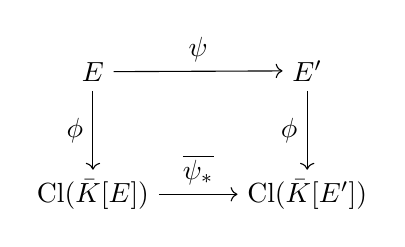
\begin{tikzpicture}
        \node (E) {$E$};
        \node[below = of E] (KE) {$\mathrm{Cl}(\bar{K}[E])$};
        \node[right = of KE] (KEp) {$\mathrm{Cl}(\bar{K}[E'])$};
        \node[above = of KEp] (Ep) {$E'$};

        \draw[->] (E) -- (Ep) node[midway, above] {$\psi$};
        \draw[->] (E) -- (KE) node[midway, left] {$\phi$};
        \draw[->] (Ep) -- (KEp) node[midway, left] {$\phi$};
        \draw[->] (KE) -- (KEp) node[midway, above] {$\overline{\psi_*}$};
    \end{tikzpicture}
    \end{center}

    Clearly this holds for $\O$, so consider $(\lambda, \mu) \in E$ with $\psi(\lambda, \mu) \neq \O$.
    As $\psi^*$ is injective, is suffices to show that $(\psi^* \circ \phi \circ \psi)(\lambda, \mu) = (\psi^* \circ \overline{\psi_*} \circ \phi)(\lambda, \mu)$.

    Using the definition of $\phi$ we find
    \begin{align*}
        &(\psi^* \circ \overline{\psi_*} \circ \phi)(\lambda, \mu) = \overline{\langle N(X - \lambda), N(Y - \mu) \rangle} \quad \text{and} \\
        &(\psi^* \circ \phi \circ \psi)(\lambda, \mu) = \psi^*\left(\overline{\langle X - \psi_1(\lambda, \mu), Y - \psi_2(\lambda, \mu) \rangle}\right)  = \overline{\langle \psi_1 - \psi_1(\lambda, \mu), \psi_2 - \psi_2(\lambda, \mu) \rangle}
    \end{align*}
    Explicitly computing the determinant of the multiplication map shows that
    \begin{equation*}
        N(X - \lambda) = \mathrm{MiPo}_{\psi^*\bar{K}(E)}(X)(\lambda) = \mathrm{MiPo}_{\bar{K}(\psi_1)}(X)(\lambda)
    \end{equation*}
    By the above, find $f, h \in \bar{K}[T]$ such that $\psi_1 = f(X)/h(X)$ and $f(T) - \psi_1h(T)$ is the minimal polynomial of $X$.
    Now we see that ($\psi(\lambda, \mu) \neq \O$ so $h(\lambda) \neq 0$)
    \begin{equation*}
        N(X - \lambda) = f(\lambda) - \psi_1h(\lambda) = -h(\lambda)(\psi_1 - \psi_1(\lambda, \mu))
    \end{equation*}
    By a similar approach one can also compute that
    \begin{equation*}
        N(Y - \mu) = -h(\lambda)(\psi_2 - \psi(\lambda, \mu))
    \end{equation*}
    So
    \begin{equation*}
        \overline{\langle N(X - \lambda), N(Y - \mu) \rangle} = \overline{\langle \psi_1 - \psi_1(\lambda, \mu), \psi_2 - \psi_2(\lambda, \mu) \rangle} \in \mathrm{Cl}(\bar{K}[E])
    \end{equation*}
    and we are done.
\end{proof}

The map $\psi^*$ considered in \ref{prop:isogeny_homomorphism} is indeed quite important, as it induces a field extension
\begin{equation*}
    \bar{K}(E) \ | \ \psi^*(\bar{K}(E'))
\end{equation*}
Using this, we can describe certain properties of isogenies.

\begin{definition}
    An isogeny $\psi: E \to E'$ is called separable, if the corresponding field extension $\bar{K}(E) | \psi^*\bar{K}(E)$ is separable.
    The degree of $\bar{K}(E) | \psi^*\bar{K}(E)$ is called the degree of $\psi$.
\end{definition}

There are many nice propositions in this context. For example, the field extension $\bar{K}(E) | \psi^*\bar{K}(E)$ is always finite, and if the isogeny is separable, then its degree is equal to $\#\ker\psi$.
This is not fundamental for the cryptosystem we consider later, but keeping it in mind helps with understanding the following theorems.

\begin{prop}
    \label{prop:unique_isogeny}
    Let $E$ be an elliptic curve and $\Phi \subseteq E$ a finite subgroup. Then there is a unique elliptic curve $E' = E/\Phi$ (up to isomorphism) and a unique separable isogeny $\phi: E \to E'$ with kernel $\Phi$.
\end{prop}
\begin{proof}
    See e.g. \cite[III.4.12]{arithmetic_elliptic_curves}.
    The proof proceeds by first constructing a field extension $\bar{K}(E)|L$ using Galois theory and then finds a morphism $\phi$ with $L = \phi^*\bar{K}(E)$.
    However, in many places the required Algebraic Geometry is beyond the scope of this work.
\end{proof}

As this curve is of fundamental importance, we introduce a new notation for it.

\begin{definition}
    Let $E$ be an elliptic curve and $G \leq E$ a finite subgroup. Then the unique elliptic curve $E'$ such that there is an isogeny $E \to E'$ with kernel $G$ is denoted by $E/G := E'$.
\end{definition}

This notation is compatible with the notation for a quotient group, as \ref{prop:isogeny_surjective} and the isomorphism theorem show that the group structure on the image Elliptic Curve matches the quotient group structure.

This last theorem is a fundamental component in the construction of isogeny based cryptosystems.
For this, a non-constructive proof as in \ref{prop:unique_isogeny} is not sufficient however, as we have to be able to compute the elliptic curve $E/\Phi$ and the corresponding isogeny efficiently.
Partly, this can be done by the famous Vélu formulas.

\begin{prop}
    \label{prop:velu_formulas}
    Let $E: y^2 = x^3 + Ax + B$ be an elliptic curve defined over $K$ and $G \leq E$ be a finite subgroup.
    Then $E/G$ is defined by $y^2 = x^3 + A'x + B'$ where
    \begin{align*}
        A' &= A - 5\sum_{(u, v) \in G \setminus \{\O\}} 3u^2 + A \\
        B' &= B - 7\sum_{(u, v) \in G \setminus \{\O\}} 5u^3 + 3Au + B
    \end{align*}
    and the isogeny $\phi: E \to E/G$ is given by
    \begin{equation*}
        \phi(P) = \left( x(P) + \sum_{Q \in G \setminus \{\O\}} x(P + Q) - x(Q), \quad y(P) + \sum_{Q \in G \setminus \{\O\}} y(P + Q) - y(Q) \right)
    \end{equation*}
    for $P \not\in G$.
    (Here $x(P)$ resp. $y(P)$ are the $x$-resp. $y$-coordinates of $P \in \bar{K}^2$)
\end{prop}
\begin{proof}
    By the uniqueness of \ref{prop:unique_isogeny} it suffices to show that the given morphism maps to this Elliptic Curve and has the specified kernel.
    This is done e.g. in \cite[8.2]{defeo_phd} by a lengthy, but mostly elementary, computation.
\end{proof}

\section{Supersingular Diffie-Hellmann}

\subsection{Supersingular Curves}

An advanced concept in the theory of Elliptic Curves is the distinction of ordinary and supersingular curves.
These notions are defined in terms of the Endomorphism ring of an Elliptic Curve.

\begin{definition}
    \label{def:endomorphism_ring}
    Let $E$ be an Elliptic Curve. Then
    \begin{equation*}
        \mathrm{End}(E) := \{ \psi: E \to E \ | \ \psi \ \text{isogeny (defined over $\bar{K}$)} \}
    \end{equation*}
    endowed with pointwise addition and composition is called the Endomorphism ring of $E$.
\end{definition}

True to its name, the Endomorphism ring is a (sometimes non-commutative) ring.

\begin{prop}
    Let $E$ be an Elliptic Curve. Then $\mathrm{End}(E)$ is a (non-commutative) ring.
\end{prop}
\begin{proof}
    Clearly the zero-map $0: P \mapsto \O$ is an isogeny and neutral w.r.t $+$.
    The identity $\mathrm{id}_E$ is also an isogeny and neutral w.r.t $\circ$.
    It is also easy to see that both $+$ and $\circ$ are associative.

    So it is left to show distributivity and the existence of inverse elements w.r.t $+$.
    Let $\psi_1, \psi_2, \rho \in \mathrm{End}(E)$. Then for all $P \in E$ have
    \begin{equation*}
        ((\psi_1 + \psi_2) \circ \rho)(P) = (\psi_1 + \psi_2)(\rho(P)) = \psi_1(\rho(P)) + \psi_2(\rho(P)) = (\psi_1 \circ \rho + \psi_2 \circ \rho)(P)
    \end{equation*}
    and
    \begin{equation*}
        \rho \circ (\psi_1 + \psi_2)(P) = \rho(\psi_1(P) + \psi_2(P)) = \rho(\psi_1(P)) + \rho(\psi_2(P)) = (\rho \circ \psi_1 + \rho \circ \psi_2)(P)
    \end{equation*}
    as $\rho$ is a group homomorphism.

    At last consider the isogeny $-1 := [X, -Y, 1]$. 
    As $-(x : y : 1) = (x : -y : 1)$ it follows that $-1 + 1 = 0$. 
    By distributivity, we get that $-1 \circ \psi$ is inverse to $\psi$ w.r.t $+$.
\end{proof}

Using this, we can define the notion of supersingular curves.

\begin{definition}
    An Elliptic Curve $E$ over a field $K$ of finite characteristic is called supersingular, if $\mathrm{End}$ is not commutative.
    Otherwise it is called ordinary.
\end{definition}

There is a lot of interesting theory on this notion. 
One usually starts by looking at the Frobenius endomorphism $\pi := [X^q, Y^q, 1] \in \mathrm{End}(E)$ where $E$ is defined over $\mathbb{F}_q$.
This theory then yields that $\mathrm{End}(E)$ is either isomorphic to an order in a quadratic imaginary number field (the ordinary case), or to a Quaternion Algebra (the supersingular case).

The Endomorphism ring is also important when examining the security of isogeny-based cryptography, but due to its complexity, we cannot present it in this work.
The interested reader might refer to \cite{arithmetic_elliptic_curves} for an introduction to this theory.
We will only require the following theorem on the group structure of supersingular Elliptic Curves.

\begin{theorem}
    \label{prop:supersingular_structure}
    Let $E$ be a supersingular Elliptic Curve defined over $\bar{\mathbb{F}}_p$ such that $j(E) \neq 0, 1728$.
    Then $E(\mathbb{F}_{p^2}) \cong (\Z / (p \pm 1)\Z)^2$.
\end{theorem}
\begin{proof}
    A slightly more general theorem is presented in \cite[Thm 54]{mathematics_isogeny_crypto}.
    For a proof, see e.g. \cite[Thm 4.2]{structure_supersingular_curve} and \cite[Lemma 4.8]{structure_supersingular_curve}.
\end{proof}

\subsection{The Isogeny Path Problem}

We already presented the Vélu formulas \ref{prop:velu_formulas} as a way to compute quotient Elliptic Curves and the corresponding isogenies.
However there is one fundamental obstacle to directly using this in a cryptosystem.
In a cryptographic scheme, the kernel subgroup will usually be of exponential size, and so a naive implementation of the Vélu formulas has infeasible running time complexity.
If the order of the kernel is smooth however (i.e. has only small prime factors), we can use the following approach.

\begin{remark}
    \label{prop:efficient_isogeny_computation}
    Let $E$ be an Elliptic Curve and $P, Q \in E$ be points.
    As isogenies are group homomorphisms, we see that $E/\langle P, Q \rangle \cong (E / \langle P \rangle) / \langle \overline{Q} \rangle$, where $\overline{Q}$ is the image of $Q$ under the canonical isogeny $E \to E/\langle P \rangle$.
    
    More generally, given a chain of subgroups
    \begin{equation*}
        \{ \O \} \leq G_1 \leq G_2 \leq ... \leq G_m \leq E
    \end{equation*}
    we have that $E/G_m \cong E/G_1/G_2'/.../G_m'$ where $G_i'$ is the image of $G_i$ under the canonical isogeny $E \to E/G_{i - 1}$.
    Computing the quotients of $E/G_1/G_2'/.../G_m'$ one after another using the Vélu formulas can now be done in
    \begin{equation*}
        \mathrm{poly}\Bigl( [\{\O\} : G_1]\ [G_1 : G_2]\ ...\ [G_{m - 1} : G_m] \Bigr)
    \end{equation*}
    operations.
\end{remark}

Because of this reason, the kernels are usually cyclic subgroups whose order is a power of 2 or 3.
For these cases, the SIKE scheme uses optimized formulas for point doubling \cite[1.1.6]{sike} and tripling \cite[1.1.7]{sike} as well as for computing isogenies with kernels of order 2 or 3 \cite[1.1.9]{sike}.
This idea leads us to another view onto isogeny problems.

\begin{definition}
    Let $p, l$ be distinct primes. 
    Then the graph whose vertices are the isomorphism classes of supersingular Elliptic Curves defined over $\bar{\mathbb{F}_p}$, and whose edges are given by the pairs of Elliptic Curves between whom there exists a separable isogeny of degree $l$, is called the supersingular $l$-isogeny graph over $\bar{\mathbb{F}_p}$.
\end{definition}

There is the notion of a dual isogeny (see e.g. \cite{arithmetic_elliptic_curves}), hence it makes sense that the graph is undirected.
An example of supersingular isogeny graphs in $\mathbb{F}_{97^2}$ is displayed in Figure~\ref{fig:isogeny_graphs}.

\begin{figure}
    \centering
    \begin{minipage}{0.49\textwidth}
        \centering
        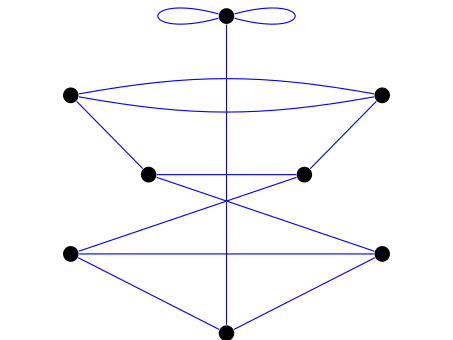
\includegraphics[width = \textwidth]{isogeny_graph1.pdf}
    \end{minipage}
    \begin{minipage}{0.49\textwidth}
        \centering
        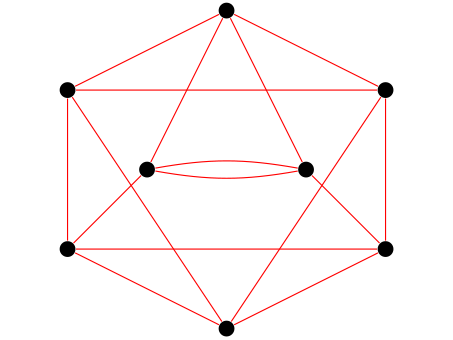
\includegraphics[width = \textwidth]{isogeny_graph2.pdf}
    \end{minipage}
    \caption{\label{fig:isogeny_graphs} supersingular 2-and 3-isogeny graphs in $\mathbb{F}_{97^2}$, from\cite{mathematics_isogeny_crypto}}
\end{figure}

Note that by the above approach, an isogeny of degree $l^e$ corresponds to a path of length $e$ is this graph.
Finding such paths is now the basic problem isogeny-based cryptography relies upon.

\begin{problem}[Supersingular Isogeny Path]
    Given two supersingular Elliptic Curves $E, E'$ defined over $\bar{\mathbb{F}_p}$ and a prime $l \neq p$, find an isogeny $\phi: E \to E'$ of degree $l^e$ for some $e \in \N$.
\end{problem}

This problem is conjectured to be extremely difficult, and the only known algorithms require time exponential in $\log \#E(\mathbb{F}_{p^2})$ \cite{mathematics_isogeny_crypto}.
Because of this, the problem (and its ordinary counterpart) seem like good candidates for building cryptographic schemes.
In the following, we will look at a kind of Diffie-Hellmann key exchange scheme.

\subsection{Supersingular Isogeny Diffie-Hellman}

The idea of the SIDH scheme is that Alice and Bob choose secret subgroups $A, B \leq E$ of a public Elliptic Curve $E$ and exchange $E/A$ resp. $E/B$.
The joint key is then $E/\langle A, B \rangle$.
To allow a short representation of $A$ and $B$, we will choose the Elliptic Curve such that Theorem~\ref{prop:supersingular_structure} applies, and then take cyclic subgroups with $\mathbb{F}_{p^2}$-rational generators.

The main problem that is left is that there is no efficient way of computing $E/\langle A, B \rangle$ given only $A$ and $E/B$.
In SIDH, this problem is solved by exchanging slightly more information about the secret isogenies $E \to E/A$ resp. $E \to E/B$.

Before we can present the cryptosystem, we require one last notation.

\begin{definition}
    Let $E$ be an Elliptic Curve defined over $\mathbb{F}_q$ and $n \in \N_{>0}$. Then
    \begin{equation*}
        E[n] := \{ P \in E(\mathbb{F}_q) \ | \ n \cdot a = \O \} \leq E
    \end{equation*}
    is the $n$-torsion subgroup of $E$.
\end{definition}

Now consider the following key exchange scheme, which is also displayed in Figure~\ref{fig:sidh}.

\begin{figure}
    \centering
    \includegraphics[width = 0.8\textwidth]{scheme2.pdf}
    \caption{\label{fig:sidh} The SIDH protocol}
\end{figure}

\begin{description}
    \item[Public data] 
        Choose primes $l_A, l_B$ such that $p := l_A^{e_A} l_B^{e_B} f \pm 1$ is prime for some (small) $f \in \N$. Now find a supersingular elliptic curve $E$ defined over $\F_q$ with $q = p^2$ and
        \begin{equation*}
            E(\F_q) \cong \left( \Z / (p \mp 1) \Z \right)^2
        \end{equation*}
        In particular, every subgroup is a free $\Z$-module of rank (at most) 2, and so we find a basis $P_A, Q_A$ of the $l_A^{e_A}$-torsion subgroup $E[l_A^{e_A}]$ of $E(\F_q)$ and similarly $P_B, Q_B$ of $E[l_B^{e_A}]$.
        \begin{center}
            The public data consists now of $l_A, e_A, l_B, e_B, E, P_A, Q_A, P_B, Q_B$
        \end{center}

    \item[Secret Generation] 
        Alice chooses a secret point $A := [m_A]P_A + [n_A]Q_A \in E[l_A^{e_A}]$ with maximal order $l_A^{e_A}$ using random $m_A, n_A \in \Z$. 
        Similarly, Bob chooses a secret point $B := [m_B]P_B + [n_B]Q_B \in E[l_B^{e_B}]$ with maximal order $l_B^{e_B}$. 
        Note that these points correspond to unique separable isogenies
        \begin{equation*}
            \alpha: E \to E_A := E/\langle A \rangle \ \text{and} \ \beta: E \to E_B := E/\langle B \rangle
        \end{equation*}
        with kernels $\langle A \rangle$ resp. $\langle B \rangle$. 
        Now they publish $E_A$ and $E_B$ and additionally $\alpha(P_B), \alpha(Q_B)$ resp. $\beta(P_A), \beta(Q_A)$.
        \begin{center}
            Secret are $m_A, n_A, m_B, n_B$ resp. $A, B, \alpha, \beta$; \\
            Public are $E_A, E_B, \alpha(P_B), \alpha(Q_B), \beta(P_A), \beta(Q_A)$
        \end{center}

    \item[Key Computation]
        Alice now computes $A' := [m_A]\beta(P_A) + [n_A]\beta(Q_A) \in E_B(\F_q)$ and the unique separable isogeny
        \begin{equation*}
            \alpha': E_B \to E_{BA} := E_B/\langle A' \rangle
        \end{equation*}
        with kernel $\langle A' \rangle$. 
        Similarly, Bob computes $B' := [m_B]\alpha(P_B) + [n_B]\alpha(Q_B)$ and the unique separable isogeny
        \begin{equation*}
            \beta': E_A \to E_{AB} := E_A/\langle B' \rangle
        \end{equation*}
        with kernel $\langle B' \rangle$. 
        \begin{center}
            Now have the joint key $j(E_{AB}) = j(E_{BA})$
        \end{center}
\end{description}
Note $l_A^{e_A}l_B^{e_B}f \pm 1$ is prime relatively often, so in the first step, we can simply try multiple choices and use a suitable one.
The isogeny computations can be done efficiently as described in \ref{prop:efficient_isogeny_computation}.
To show correctness, it suffices now to show that $j(E_{AB}) = j(E_{BA})$.
\begin{proof}
    As $B' = \alpha(B)$ have $\alpha^{-1}(\{B'\}) = \ker(\alpha) + B = \langle A \rangle + B$.
    Hence
    \begin{equation*}
        \ker(\beta' \circ \alpha) = \alpha^{-1}(\ker(\beta')) = \alpha^{-1}(\langle B' \rangle) = \langle A + \langle B \rangle \rangle = \langle A, B \rangle
    \end{equation*}
    Similarly get that $\ker(\alpha' \circ \beta) = \langle A, B \rangle$. Now \ref{prop:unique_isogeny} yields that $E_{AB} \cong E_{BA}$ and thus they have the same j-invariant.
    Up to isomorphism, this is shown by the following commutative diagram:
    \begin{center}
        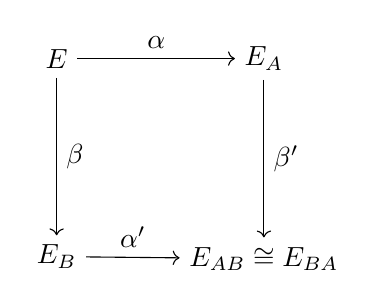
\begin{tikzpicture}[node distance = 2cm]
            \node (E) {$E$};
            \node (EA) [right = of E] {$E_A$};
            \node (EB) [below = of E] {$E_B$};
            \node (EAB) [below = of EA] {$E_{AB} \cong E_{BA}$};
            \draw [->] (E) -- node [above, midway] {$\alpha$} (EA);
            \draw [->] (E) -- node [right, midway] {$\beta$} (EB);
            \draw [->] (EA) -- node [right, midway] {$\beta'$} (EAB);
            \draw [->] (EB) -- node [above, midway] {$\alpha'$} (EAB);
        \end{tikzpicture}
    \end{center}
\end{proof}

As with classical Diffie-Hellman, no reduction to the Isogeny Path problem is known (comparable to the Discrete Logarithm problem in the classical case).
For SIDH, the situation is even worse, as it is required to additionally publish the values $\alpha(P_B), \alpha(Q_B)$ and $\beta(P_A), \beta(Q_A)$.
It is still not well understood how this influences the security of the scheme.
However, the scheme is known for almost a decade now and not been broken.
In fact, the algorithms breaking SIDH have not even improved significantly and the initial security estimates remain valid.

\subsection{Supersingular Isogeny Key Encapsulation}

Supersingular Isogeny Key Encapsulation (SIKE) is the name of the (alternative) NIST candidate that is based on SIDH.
In the following, we will outline some of its less theoretical features.
A more detailed overview is given in the specification document \cite{sike}.

The core of SIKE is an implementation of SIDH, that uses various techniques for optimization.
Most important among those is the representation of points using only three x-coordinates.
Concretely, instead of publishing $\alpha(P_B), \alpha(Q_B)$ Alice transmits the x-coordinates of $\alpha(P_B), \alpha(Q_B), \alpha(P_B - Q_B)$ and similar for Bob.
Elliptic Curves are also represented by their Montgomery form, i.e. by a defining equation of the form $bY^2 = X^3 + aX^2 + x$.
Interestingly, the x-coordinates of $\alpha(P_B), \alpha(Q_B), \alpha(P_B - Q_B)$ are already sufficient for determining $E/\langle A \rangle$ (up to isomorphism).
The reason is that the j-invariant of a curve in Montgomery form is
\begin{equation*}
    j(E) = \frac {256(a^2 - 3)^3} {a^2 - 4} \quad \text{(if $a^2 \neq 4$)}
\end{equation*}
which does not depend on $b$ \cite[1.1.8]{sike}.
Because of this, the public key size of SIDH-based schemes is extremely low.
On the other hand, the running time is more than an order of magnitude slower than the one of other PQC candidates.

Based on SIDH, SIKE then defines an encryption protocol à la ElGamal.
Finally, a variant of the Fujisaki-Okamoto transform by \cite{kem_transform} is used on top of the encryption scheme to provide an IND-CCA secure key encapsulation scheme.
Both of these construc-tions are standard and have nothing to do with Elliptic Curves.

The SIKE submission provides four sets of parameters for different security levels.
All of them use the curve $E_0: y^2 = x^3 + 6x^2 + x$ defined over $\mathbb{F}_{p^2}$, albeit with different $p$ as displayed in Table~\ref{tab:sike_statistics}.

\begin{figure}
    \centering
    \begin{tabular}{ r | c c c c }
        & SIKEp434 & SIKEp503 & SIKEp610 & SIKEp751 \\
        \hline\\
        bitlength of $p$ & 434 & 503 & 610 & 751 \\
        $e_A$ & 216 & 250 & 305 & 372 \\
        $e_B$ & 137 & 159 & 192 & 239 \\
        Key Generation cycles & $5.9 \cdot 10^6$ & $8.2 \cdot 10^6$ & $1.5 \cdot 10^7$ & $2.5 \cdot 10^7$ \\
        Key Encapsulation cycles & $9.7 \cdot 10^6$ & $1.4 \cdot 10^7$ & $2.7 \cdot 10^7$ & $4.1 \cdot 10^7$ \\
        Key Decapsulation cycles & $1.0 \cdot 10^7$ & $1.4 \cdot 10^7$ & $2.7 \cdot 10^7$ & $4.4 \cdot 10^7$ \\
        Public Key size (bytes) & 330 & 378 & 462 & 564 \\
        Secret Key size (bytes) & 374 & 434 & 524 & 644 \\
        Ciphertext size (bytes) & 346 & 402 & 486 & 596 \\
        Shared secret size (bytes) & 16 & 24 & 24 & 32 \\
        Estimated security level (bits) & 142 & 169 & 209 & 263
    \end{tabular}
    \caption{\label{tab:sike_statistics} Statistics on the different parameter sets of SIKE from \cite{sike}; Performance was measured on a 3.4GHz Intel i7-6700 using an optimized assembly implementation for x64}
\end{figure}

\printbibliography

\end{document}